\chapter{Dinamica del corpo rigido}
Un corpo rigido è un sistema di punti materiali in cui le distanze tra tutte le possibili coppie di punti non possono variare. Chiaramente, il corpo rigido è un modello ideale, quello del corpo indeformabile, al quali si avvicinano i corpi solidi ordinari, nella pratica sempre deformabili. Nel moto di un corpo rigido è possibile individuare un moto d'insieme, riconducibile al moto del centro di massa, il quale è in una posizione immutabile rispetto a tutti i punti del corpo rigido, date le caratteristiche di quest'ultimo. Tuttavia, è facile vedere come i vari punti che compongono il corpo possano descrivere traiettorie diverse tra loro e da quella del centro di massa. Questo significa che il moto d'insieme non contiene e non può rappresentare tutta la dinamica del corpo rigido, ovvero che questo non può essere trattato come se fosse un punto materiale. Quindi, per studiare la dinamica del corpo rigido è necessario il sistema di riferimento del centro di massa del corpo rigido; poiché la distanza dei singoli punti non cambia mai, ciascun punto è visto dal centro di massa o in quiete o in moto lungo un arco di circonferenza. Inoltre, si può considerare un sistema di riferimento $(x^*,y^*,z^*)$ con gli assi solidali al corpo rigido. Tale sistema, in cui ciascun punto è fermo, è utile per visualizzare il moto del corpo rigido rispetto agli altri due sistemi di riferimento (quello inerziale e quello del centro di massa). 

Un corpo rigido è formato da $n$ punti, i quali possono essere un insieme discreto o distribuiti con continuità, in ogni caso è un corpo esteso. Il suo moto è determinato dalle forze esterne che, in generale, sono più di una e possono essere applicate in punti diversi. Si parla quindi di sistemi di forze con una risultante $\Rext$ e un momento $\Mext$, indipendenti tra di loro. In un corpo rigido, il lavoro delle forze interne è nullo, $W^{int}=0$, dato che i punti mantengono invariate le distanze mutue. Pertanto, la variazione di energia dell'energia cinetica di un corpo rigido è uguale al lavoro delle sole forze esterne. Dunque, le leggi fondamentali della dinamica del corpo rigido sono
\begin{equation}
    \vR=m\acm,\quad\vM=\frac{d\vL}{dt},\quad\Delta K=W.
\end{equation}
\begin{notz}
    In questo capitolo si tralascia l'apice ``ext'' per le grandezze $\vR$, $\vM$ e $W$ dato che non può esserci confusione. 
\end{notz}

\section{Proprietà del corpo rigido}
Un corpo esteso appare avere una struttura continua rispetto a qualsiasi suddivisione macroscopica, d'altra parte è noto che qualsiasi corpo esteso è costituito da molecole o atomi. Il singolo punto materiale va quindi pensato come un volume $dV$ contenente una massa $dm$. Il volume $dV$ è piccolo rispetto alla scala macroscopica, ma piccolo grande a quella microscopica. Questa suddivisione permette di estendere al continuo i risultati trovati per i sistemi discreti di punti materiali. Questo passaggio implica la sostituzione delle somme con gli integrali, pertanto è possibile usare tutte le proprietà del calcolo integrale per determinare certe grandezze. 
\begin{obs}
    Il fatto che questa suddivisione ignori l'effettiva composizione atomica del corpo è irrilevante ai fini dello studio della dinamica macroscopica. 
\end{obs}
Si definisce la densità $\rho$ del corpo rigido come il rapporto
\begin{equation}
    \rho=\frac{dm}{dV}.
\end{equation}
Anche supponendo che i volumi infinitesimi siano tutti uguali, non è ovvio che ciascuno contenga la stessa quantità di massa. Da questa definizione, la massa del corpo rigido è espressa in termini della funzione densità, quindi
\begin{equation}
    m=\int dm=\int_V\rho(x,y,z)\,dV.
\end{equation}
Un corpo del quale la densità è costante viene detto omogeneo. In tal caso, la sua massa è
\begin{equation}
    m=\rho V.
\end{equation}
I corpi in cui questo non avviene sono detti non omogenei. In questi casi è comunque possibile definire la densità media come $\bar{\rho}=m/V$. 

Nel caso la massa sia distribuita su una superficie o una lunghezza, invece che su un volume, si definiscono la densità superficiale $\rho_S$ e la densità lineare $\rho_L$ come
\begin{equation}
    \rho_S=\frac{dm}{dS},\quad\rho_L=\frac{dm}{dl}.
\end{equation}
La grandezza $v=1/\rho$ prende il nome di volume specifico: mentre la densità può essere pensata come la massa contenuta nell'unità di volume, il volume specifico rappresenta il volume occupato dall'unità di massa. 

Dato che la posizione di ciascun punto di un corpo rigido di massa $dm=\rho\,dV$ è individuata da un raggio vettore $\vr$, la posizione del centro di massa, in analogia con quanto detto per i sistemi discreti di punti, è
\begin{equation}
    \rcm=\frac{\int\vr\,dm}{\int dm}=\frac{\int_V\vr\rho\,dV}{\int_V\rho\,dV}=\frac{1}{m}\int_V\vr\rho\,dV.
\end{equation}
Se il corpo è omogeneo, $\rcm$ è
\begin{equation}
    \rcm=\frac{\rho}{m}\int\vr\,dV=\frac{1}{V}\int\vr\,dV.
\end{equation}
Da questa espressione è evidente che la posizione del centro di massa di un corpo rigido omogeneo è la media integrale della funzione vettoriale $\vr(x,y,z)$ nel volume $V$, non dipende dal valore della massa del corpo, ma solo dalla sua forma. Ad esempio, il centro di massa di un'asta omogenea è sempre nel centro qualunque sia il materiale costituente. Anche se meno evidente, ciò continua ad essere vero per un corpo non omogeneo se la distribuzione di massa è la stessa indipendentemente dal materiale costituente. 
\begin{obs}
    In generale, $\vr=\vr(x,y,z)$ e $\rho=\rho(x,y,z)$ sono funzioni dipendenti dalle coordinate ed anche $dV=dxdydz$ è esprimibile in questi termini. 
\end{obs}
In generale, se un corpo omogeneo è simmetrico rispetto ad un punto o ad un piano, il centro di massa rispettivamente coincide con il centro di simmetrica o è un punto sull'asse o del piano di simmetria. Se esistono più assi o piani di simmetria, allora il centro di massa sta sulla loro intersezione. 

Si consideri un corpo continuo soggetto alla forza peso. Su ciascun elemento agisce la forza $\vg\,dm$ e la risultante di tutte queste forze parallele è
\begin{equation}
    \int\vg\,dm=\vg\int dm=m\vg,
\end{equation}
applicata nel centro di massa. Rispetto ad un polo fisso, che potrebbe essere l'origine delle coordinate, il momento risultante è
\begin{equation}
    \vM=\int\vr\times\vg\,dm=\bigg(\int\vr\,dm\bigg)\times\vg=m\rcm\times\vg=\rcm\times m\vg,
\end{equation}
il quale è uguale al momento della risultante, ossia della forza peso, rispetto allo stesso polo. L'energia potenziale quindi è
\begin{equation}
    U(z)=\int g z\,dm=g\int z\,dm=mg\zcm.
\end{equation}
Se il corpo è libero e agisce solo la forza peso, la traiettoria del centro di massa è verticale rettilinea oppure parabolica a seconda delle condizioni iniziali.

\section{Moto del corpo rigido}
Per determinare quale sia il moto più generale di un corpo rigido si deve prima partire dallo studio di due moti più semplici: la traslazione e la rotazione. 

Nel moto di traslazione tutti i punti descrivono traiettorie uguali, in generale curvilinee, percorse con la stessa velocità $\vv$, che può variare nel tempo in modulo, direzione e verso. Tale $\vv$ coincide con $\vcm$. Pertanto, nel moto di traslazione, che può essere uniforme o vario, se è noto il moto del centro di massa è noto anche quello di qualsiasi altro punto. La dinamica è quella di un punto materiale e non c'è movimento rispetto al centro di massa, quindi
\begin{equation}
    \vL'=0,\quad K'=0.
\end{equation}
Le grandezze significative sono: la quantità di moto $\vp=m\vcm$ e l'energia cinetica $K=K_{CM}=m\vcm^{\ 2}/2$. L'equazione del centro di massa è
\begin{equation}
    \vR=m\acm.
\end{equation}
Il momento angolare si ricava dalla conoscenza di $\vp$ e $\rcm$, infatti
\begin{equation}
    \vL=\vL_{CM}=\rcm\times m\vcm=\rcm\times\vp.
\end{equation}
Da ciò si vede che $\vL$ non è indipendente da $\vp$. Di conseguenza, anche l'equazione $\vM=d\vL/dt$ non aggiunge alcuna informazione.

Nel moto di rotazione tutti i punti descrivono un moto circolare, le traiettorie sono archi di circonferenze diverse che stanno su piani tra loro paralleli e hanno il centro sull'asse di rotazione.
L'equazione del moto di rotazione è
\begin{equation}
\label{eq: eq. moto rotazione corpo rigido}
    \vM=\frac{d\vL}{dt}.
\end{equation}
La rigidità del corpo implica che tutti i punti abbiano in un dato istante la stessa velocità angolare $\vom$, che è parallela all'asse di rotazione; le velocità $\vv$ dei singoli punti sono diverse, a seconda della distanza $R_i$ dall'asse di rotazione, in modulo $v_i=\omega R_i$. Se l'asse di rotazione è fisso nel tempo $\vom$ può cambiare solo in modulo e verso e si ha un moto circolare vario, che è uniforme se $\vom$ è costante. In generale, $\vom$ può cambiare anche in direzione. 

In conclusione, i due tipi di moto considerati sono gli unici da studiare in dettaglio dato che si dimostra che il moto di un corpo rigido è in generale una rototraslazione: ogni spostamento infinitesimo può essere essere considerato come somma di una traslazione e di una rotazione infinitesime, individuate da $\vv$ e $\vom$ variabili nel tempo. 

\subsection{Rotazioni rigide attorno ad un asse fisso}
Si consideri la rotazione di un corpo rigido attorno ad un asse fisso in un sistema di riferimento inerziale. I punti dell'asse di rotazione sono fissi e quindi possono essere utilizzati come poli per il calcolo dei momenti. Inoltre, l'asse di rotazione può essere esterno al corpo e il centro di massa non è detto che sia un punto dell'asse stesso. Il vettore $\vom$ ha direzione fissa, quella dell'asse di rotazione, mentre il suo modulo è in generale variabile nel tempo. Il verso di $\vom$ indica il verso della rotazione. Se $\vom$ varia, il vettore accelerazione angolare $\alpha=d\vom/dt$ è diverso da zero, anch'esso parallelo all'asse di rotazione. Si ricordi che in una rotazione rigida ciascun punto $P_i$ descrive in un piano ortogonale all'asse di rotazione una traiettoria circolare con centro sull'asse e raggio $R_i$ pari alla distanza di $P_i$ dall'asse. La velocità del punto è $\vv_i$, di modulo $\omega R_i$, mentre l'accelerazione è $\va_i$, con componente normale $\omega^2R_i$ e tangente $\alpha R_i$. 

Si assuma, con riferimento alla figura \ref{fig: rotazione rigida}, che l'asse $z$ sia l'asse di rotazione, quindi $\vom$ è parallelo all'asse $z$. Il raggio vettore $\vr_i$ del punto $P_i$ forma un angolo $\theta_i$ con l'asse $z$ e un angolo di $\pi/2$ con $\vv_i$. Dalla stessa figura si nota come la traiettoria abbia raggio $R_i=r_i\sin{\theta}$. Il momento angolare del punto $P_i$ rispetto al polo $O$ è dato da $\vL_i=\vr_i\times m_i\vv_i$, il quale forma un angolo $\pi/2-\theta$ con l'asse $z$. Il modulo di $\vL_i$ è
\begin{equation}
    L_i=m_ir_iv_i=m_ir_iR_i\omega.
\end{equation}
\begin{figure}[h]
    \centering
    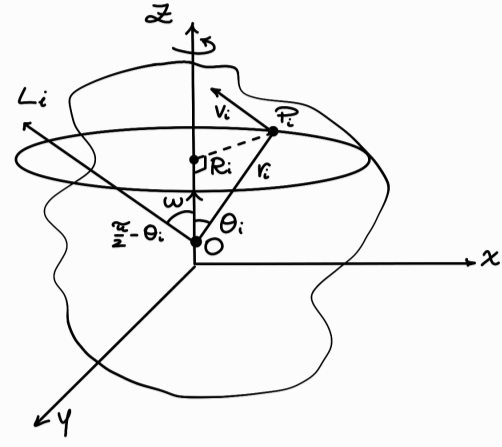
\includegraphics[width=0.5\linewidth]{Immagini/rotazioni rigide.png}
    \caption{vettore momento angolare per una rotazione rigida.}
    \label{fig: rotazione rigida}
\end{figure}

La proiezione angolare di $\vL_i$ sull'asse di rotazione, che prende il nome di momento assiale, è
\begin{equation}
    L_{iz}=L_i\cos{\bigg(\frac{\pi}{2}-\theta\bigg)}=L_i\sin{\theta_i}=m_ir_iR_i\omega\sin{\theta_i}=m_iR_i^2\omega.
\end{equation}
Il momento angolare del corpo è $\vL=\sum_i\vL_i$, e, in generale, non è parallelo all'asse di rotazione. Questo implica che in generale non esiste una proporzionalità tra $\vL$ e $\vom$. La proiezione di $\vL$ sull'asse $z$ è
\begin{equation}
    L_z=\nsum_iL_{iz}=\bigg(\nsum_im_iR_i^2\bigg)\omega=I_z\omega.
\end{equation}
Il coefficiente $I_z$ prende il nome di momento di inerziale del corpo rigido rispetto all'asse $z$ ed è appunto dato da
\begin{equation}
\label{eq: momento di inerzia discreto}
    I_z=\nsum_im_iR_i^2=\nsum_im_i(x_i^2+y_i^2).
\end{equation}
Il momento di inerzia dipende dalle masse e dalla loro posizione rispetto all'asse di rotazione: non è una caratteristica del corpo che si possa calcolare nota la sua struttura, ma per definirlo è necessario conoscere anche la posizione rispetto al corpo dell'asse di rotazione. Quindi, la componente parallela all'asse può variare solo in modulo, è proporzionale a $\omega$ e non dipende dalla scelta del polo. Invece, la componente ortogonale all'asse $L_\perp$ varia in direzione, in modulo e dipende dalla scelta del polo; questa corrisponde alla somma vettoriale di contributi, ognuno dei quali vale in modulo
\begin{equation}
    L_{i,\perp}=L_i\cos{\theta_i}=m_ir_iR_i\cos{\theta_i}.
\end{equation}
Il momento angolare $\vL$ è sicuramente parallelo all'asse di rotazione, e quindi ad $\vom$, quando l'asse di rotazione è un asse di simmetria, o, più in generale, quando l'asse di rotazione coincide con un asse principale di inerzia. In tali condizioni, si hanno
\begin{equation}
\label{eq: relazioni momento angolare per asse rot. = asse princip. inerzia}
    \vL=I_z\vom,\quad L=L_z,\quad L_\perp=0.
\end{equation}
Se $\vL$ è variabile, le variazioni $d\vL/dt$ sono anch'esse parallele a $\vom$ e quindi il momento delle forze esterne $\vM$ che le provoca è parallelo a $\vom$. Se invece $\vL$ è costante, ovvero $\vom$ è costante, il moto si svolge senza momento esterno, salvo la presenza di attrito. Nel caso più semplice in cui $\vL\parallel\vom$, valgono le \eqref{eq: relazioni momento angolare per asse rot. = asse princip. inerzia}, per cui
\begin{equation}
    \frac{d\vL}{dt}=\frac{d}{dt}(I_z\vom)=I_z\frac{d\vom}{dt}=I_z\valpha.
\end{equation}
Dunque, l'equazione del moto di rotazione è
\begin{equation}
\label{eq: moto rotazione asse rot. = asse princip. inerzia}
    \vM=I_z\valpha.
\end{equation}
Sia $\valpha$ che $\vM$ sono paralleli all'asse di rotazione, ossia a $\vom$. Note le condizioni iniziali, cioè la velocità e la posizione iniziali angolari, da \eqref{eq: moto rotazione asse rot. = asse princip. inerzia} si può ricavare la legge oraria, infatti
\begin{equation}
    \alpha=\frac{M}{I_z}\Rightarrow\omega(t)=\omega_0+\int_0^t\alpha\,dt\Rightarrow\theta(t)=\theta_0+\int_0^t\omega\,dt.
\end{equation}
Se $M=0$ il corpo resta in quiete o si muove con moto circolare uniforme, in particolare
\begin{equation}
    \alpha=0,\quad\omega=\omega_0,\quad\theta=\theta_0+\omega t.
\end{equation}
Se $M=costante$ il moto è circolare uniformemente accelerato, in particolare
\begin{equation}
    \alpha=costante,\quad\omega=\omega_0+\alpha t,\quad\theta=\theta_0+\omega_0t+\frac{1}{2}\alpha t^2.
\end{equation}
Infine, con $M$ generico, $\alpha=\alpha(t)$ e il moto è circolare vario. Per quanto riguarda in particolare il moto del centro di massa, se questo non sta sull'asse di rotazione, ma ne dista $R_{CM}$, l'accelerazione $\acm$ si calcolo a partire da $\alpha$ e $\omega$. In particolare, la componente tangente è $\acm^{T}=\alpha R_{CM}$, quella normale è $\acm^N=\omega^2R_{CM}$. La velocità è $\vcm=\omega R_{CM}$. Invece, l'energia cinetica del corpo rigido in rotazione è data da
\begin{equation}
\label{eq: energia cinetica rotazione corpo rigido}
    K=\nsum_i\frac{1}{2}m_iv_i^2=\nsum_i\frac{1}{2}m_iR_i^2\omega^2=\frac{1}{2}I_z\omega^2.
\end{equation}
Anche l'energia cinetica dipende dal momento di inerzia rispetto all'asse di rotazione. Se $\vL\parallel\vom$, allora da \eqref{eq: relazioni momento angolare per asse rot. = asse princip. inerzia} si ha
\begin{equation}
    K=\frac{L^2}{2I_z}.
\end{equation}
Quando un corpo rigido in quiete o in rotazione viene portato a ruotare con una velocità angolare $\omega_f$ tramite l'applicazione di un momento esterno, l'energia cinetica subisce una variazione e quindi è stato applicato un lavoro. Tale lavoro è dato da
\begin{equation}
\label{eq: lavoro rotazione corpo rigido}
    W=\Delta K=\frac{1}{2}I_z(\omega^2_f-\omega^2_i).
\end{equation}
Scrivendo questa equazione in forma infinitesima si ha
\begin{equation}
    dW=dK=I_z\omega\,d\omega=I_z\frac{d\theta}{dt}\alpha\,dt=I_z\alpha\,d\theta=M\,d\theta,
\end{equation}
la quale integrata dalla posizione iniziale a quella finale restituisce 
\begin{equation}
    W=\int_0^\theta M\,d\theta.
\end{equation}
Quindi, la potenza istantanea è
\begin{equation}
    P=\frac{dW}{dt}=M\frac{d\theta}{dt}=M\omega.
\end{equation}
Per eseguire il calcolo del lavoro è necessario conoscere la dipendenza angolare del momento.

Si noti che le formule \eqref{eq: relazioni momento angolare per asse rot. = asse princip. inerzia} e \eqref{eq: moto rotazione asse rot. = asse princip. inerzia} valgono solo se $\vL\parallel\vom$. In caso contrario, il vettore $\vL$ ruota intorno all'asse di rotazione descrivendo un moto di precessione, in particolare di precessione uniforme se $\vom$ è costante. In questo caso, l'equazione del moto \eqref{eq: eq. moto rotazione corpo rigido} ha due componenti 
\begin{equation}
    \vM_z=\frac{d\vL_z}{dt},\quad\vM_\perp=\frac{d\vL_\perp}{dt},
\end{equation}
essendo $\vM_z$ e $\vM_\perp$ la componente del momento angolare delle forze esterne $\vM$ parallela e perpendicolare all'asse di rotazione. La prima equazione corrisponde a \eqref{eq: moto rotazione asse rot. = asse princip. inerzia}, e da questa tramite $\alpha$ e le condizioni iniziali si ricava la legge oraria vista in precedenza: il moto di rotazione è ancora regolato da $M_z$. In particolare, se $M_z=0$, il corpo ruota con $\omega$ costante e $L_z$ è anch'esso costante. Invece, $L_\perp$ in ogni caso ruota assieme al corpo, potendo restare di modulo costante, se $\omega$ è costante, ma variando sempre in direzione. Le variazioni di $L_\perp$ sono regolate da $M_z$. In generale, la strada da seguire è:
\begin{quote}
    ``quando un corpo rigido ruota attorno ad una asse è conveniente mettersi in una situazione tale che $\vL$ e $\vom$ siano paralleli.''
\end{quote}
\begin{ex}
    Per capire l'origine di $M_\perp$ si può considerare un corpo rigido formato da due masse uguali $m$ collegate da un'asta rigida di massa trascurabile che forma un angolo $\theta$ con l'asse di rotazione. Questo ruota con velocità angolare $\vom$ e questo moto è dovuto ad un momento $M_z$, eventualmente nullo se $\vom$ è costante. D'altra parte, le due masse descrivono un moto circolare e per questo sono necessarie due forze centripete $\vF_C$, esercitate dell'asta. Queste due forze costituiscono una coppia e si dimostra che il momento è proprio $dL_\perp/dt$. Le due forze peso invece hanno momento nullo rispetto al polo $O$, come si deduce dalla figura \ref{fig: asta con masse}. 
    \begin{figure}[h]
        \centering
        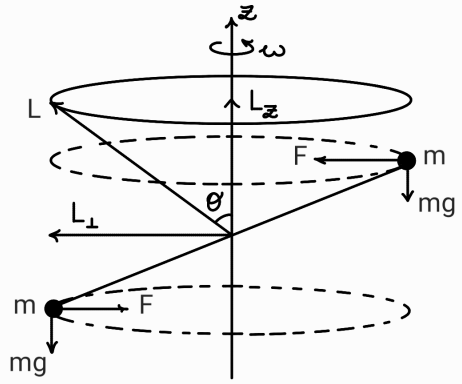
\includegraphics[width=0.5\linewidth]{Immagini/asta con masse.png}
        \caption{asta rigida in rotazione rigida.}
        \label{fig: asta con masse}
    \end{figure}
    Un effetto del momento delle $\vF_C$ è quello di far cambiare direzione all'asse di rotazione e quindi occorrono opportuni supporti in modo da mantenere l'asse in posizione verticale, i quali vengono sollecitati durante il moto. Se $\theta=\pi/2$, $\vL$ sarebbe parallelo a $\vom$ e questi effetti non si verificherebbero. 
\end{ex}
Per quanto riguarda energia cinetica e lavoro le equazioni \eqref{eq: energia cinetica rotazione corpo rigido} e \eqref{eq: lavoro rotazione corpo rigido} hanno validità generale. Invece, cambia il legame tra energia cinetica e momento angolare che diventa
\begin{equation}
    K=\frac{L_z^2}{2I_z}.
\end{equation}
Cambia anche l'espressione del lavoro tramite il momento $M_z$ che diventa
\begin{equation}
    W=\int_0^\theta M_z\,d\theta.
\end{equation}
Pertanto, quando $\vL$ non è parallelo a $\vom$, la legge oraria e il lavoro dipendono dalle componenti lungo l'asse di rotazione del momento angolare e del momento delle forze. Si vede come le corrispondenti formule nel caso del parallelismo tra $\vL$ e $\vom$ siano comprese nel caso generale, in quanto $M_z=M$ e $L_z=L$. 

\subsection{Momento di inerzia}
Il momento di inerzia ha un ruolo fondamentale, analogo a quello della massa nel secondo principio di Newton: a parità di momento applicato un corpo assume un'accelerazione angolare maggiore o minore a seconda del valore del momento di inerzia rispetto all'asse di rotazione. Tuttavia, c'è una profonda differenza tra i due concetti: mentre si può associare ad ogni corpo una massa, non ha senso parlare di momento di inerzia di un corpo di determinata forma, ma bisogna sempre specificare l'asse di rotazione a cui si fa riferimento. 

Il momento di inerzia di un corpo continuo si deduce da \eqref{eq: momento di inerzia discreto} effettuando il passaggio al continuo, quindi questo è
\begin{equation}
    I=\int R^2\,dm=\int_V\rho R^2\,dV=\int_V\rho(x^2+y^2)\,dV,
\end{equation}
dove $R$ è la distanza dell'elemento di massa $dm$ dall'asse $z$, assunto come asse di rotazione. Essendo il momento di inerzia additivo, se si suddivide un corpo in tante parti il momento di inerzia totale è la somma dei momenti di inerzia parziali, calcolati tutti rispetto allo stesso asse di rotazione. 
\begin{ex}
    Si consideri un disco omogeneo di massa $m$ e raggio $R$. La massa del disco è quindi esprimibile in termini di densità come $m=\rho_S\pi R^2$. Quindi, il momento di inerzia $I$ rispetto all'asse $z$ è
    \begin{equation}
        I_z=\int r^2\,dm=\int\rho_S r^2\,dS.
    \end{equation}
    Usando le coordinate polari $dS=r\,drd\phi$. Pertanto, si ha
    \begin{equation}
        I_z=\int\rho_S r^2\,dS=\rho_S\int_0^R\int_0^{2\pi}r^3\,drd\phi=\frac{1}{2}\pi\rho_SR^4=\frac{1}{2}mR^2.
    \end{equation}
\end{ex}
\begin{ex}
    Si consideri un'asta omogenea di massa $m$, lunghezza $d$ e sezione $S$. La massa dell'asta in termini di densità è $m=\rho Sd$, quindi un elemento infinitesimo a distanza $dx$ dall'asse è $dm=\rho S\,dx$. Quindi, il momento di inerzia rispetto ad un asse ortogonale all'asta passante per il suo centro è
    \begin{equation}
        I_z=\int_{-d/2}^{d/2}x^2\,dm=\rho S\int_{-d/2}^{d/2}x^2\,dx=\frac{1}{12}\rho Sd^3=\frac{1}{12}md^2.
    \end{equation}
    Invece, il momento di inerzia rispetto ad un asse passante per un estremo dell'asta è
    \begin{equation}
        I_z=\int_0^dx^2\,dm=\rho S\int_0^dx^2\,dx=\frac{1}{3}\rho Sd^3=\frac{1}{3}md^2.
    \end{equation}
\end{ex}
In generale, il momento di inerzia ha un'espressione del tipo 
\begin{equation}
    I=fmd^2,
\end{equation}
dove $m$ è la massa del corpo, $d$ una dimensione significativa (ad esempio il raggio per una sfera o la lunghezza per un'asta) e $f$ è un fattore numerico legato alla struttura del sistema. Pertanto, il momento di inerzia si può scrivere come
\begin{equation}
    I=mk^2,\quad k=d\sqrt{f}=\sqrt{\frac{I}{m}},
\end{equation}
dove $k$ è il raggio giratore del corpo. Dato un corpo con momento di inerzia $I$ rispetto ad un asse, si immagini di concentrarne la massa in un punto: $k$ rappresenta la distanza dall'asse a cui bisogna porre questo punto per avere lo stesso momento di inerzia $I$.

Se per il calcolo del momento di inerzia si dovesse scegliere un asse per il quale vengono meno le condizioni di simmetria, il calcolo dei vari integrali può risultare complicato. Il seguente teorema semplifica enormemente il problema. 
\begin{teo}[teorema di Huygens-Steiner]
    Il momento di inerzia di un corpo di massa $m$ rispetto ad un asse che si trova ad una distanza $a$ dal centro di massa del corpo è dato da
    \begin{equation}
        I=I_{CM}+ma^2,
    \end{equation}
    dove $I_{CM}$ è il momento d'inerzia del corpo rispetto ad un asse parallelo al primo e passante per il centro di massa.
\end{teo}
\begin{proof}
    In riferimento alla figura \ref{fig: THS proof}, si considerino due assi $z$ e $z'$, tra loro paralleli, distanti $a$. L'asse $z'$ passa per il centro di massa. La relazione tra le coordinate nei due sistemi, con centro in $O$ e nel centro di massa, è dato da
    \begin{equation}
        x=x',\quad y=y'+a,\quad z=z'.
    \end{equation}
    \begin{figure}[h]
        \centering
        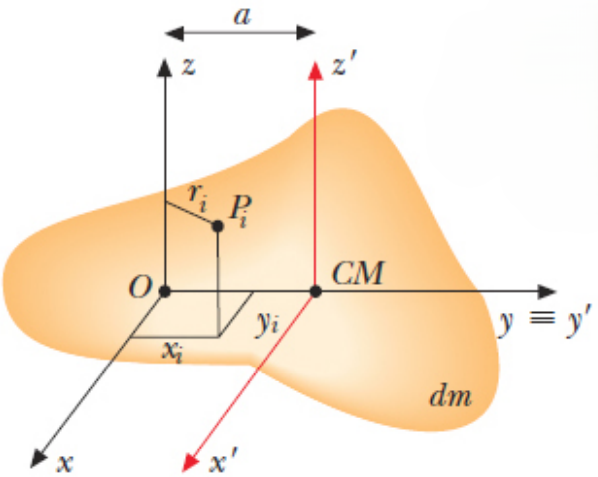
\includegraphics[width=0.4\linewidth]{Immagini/THS proof.png}
        \caption{schema per la dimostrazione del teorema di Huygens-Steiner.}
        \label{fig: THS proof}
    \end{figure}
    
    Il momento d'inerzia di un punto generico $P_i$ rispetto all'asse $z$ è dato da
    \begin{equation}
        I_{i}=m_i(x_i^2+y_i^2).
    \end{equation}
    Sommando su tutti i punti utilizzando le formule di trasformazione si ha
    \begin{equation}
        \begin{split}
            I_z&=\nsum_im_i(x_i^2+y_i^2)=\nsum_im_i[(x_i')^2+(y_i'+a)^2]\\
            &=\nsum_im_i[(x_i')^2+(y_i')^2]+\nsum_im_ia^2+2a\nsum_im_iy_i'.
        \end{split}
    \end{equation}
    Il primo termine è il momento di inerzia del corpo rispetto all'asse $z'$, il secondo è $ma^2$ e il terzo è nullo in quanto corrisponde a $m\ycm'$ e $\ycm'$, coordinata del centro di massa nel sistema del centro di massa, che è nulla. Si è quindi trovato
    \begin{equation}
         I_z=I_{z'}+ma^2=I_{CM}+ma^2.
    \end{equation}
\end{proof}
\begin{obs}
    Quindi $a$ non è altro che la distanza tra i due assi rispetto ai quali vengono calcolati i momenti d'inerzia.
\end{obs}
Si riconsideri l'equazione \eqref{eq: energia cinetica rotazione corpo rigido} e si applichi il teorema di Huygens-Steiner
\begin{equation}
    K=\frac{1}{2}(I_{CM}+ma^2)\omega^2=\frac{1}{2}I_{CM}\omega^2+\frac{1}{2}ma^2\omega^2.
\end{equation}
D'altra parte, $a\omega$ rappresenta la velocità $\vcm$, che percorre una traiettoria circolare di raggio $a$ rispetto all'asse $z$, quindi 
\begin{equation}
    K=\frac{1}{2}I_{CM}\omega^2+\frac{1}{2}m\vcm^{\ 2}.
\end{equation}
Questo risultato è in accordo con il secondo teorema di K\"onig e con le caratteristiche del moto di un corpo rigido: quando il centro di massa non è sull'asse di rotazione, l'energia cinetica è data dalla somma di $K'=I_{CM}\omega^2/2$, tipico della rotazione che costituisce il moto rispetto al centro di massa, e di $K_{CM}=m\vcm^{\ 2}/2$, energia cinetica del centro di massa. 

\subsection{Moto di puro rotolamento}
Si consideri la situazione in cui l'asse di rotazione non sia una asse materiale, ma un asse geometrico che si sposta insieme al corpo rigido. Questo si trova sopra ad un piano e si muove rispetto ad esso. Se le velocità di tutti i punti sono uguali tra loro e parallele al piano il moto è di traslazione. In generale, però il corpo in questione rotola sul piano e il punto di contatto $C$ ha velocità non nulla rispetto al piano, in tal caso il moto è di rotolamento e strisciamento. Se invece la velocità di $C$ è nulla, allora il moto è di puro rotolamento. 
\begin{figure}[h]
    \centering
    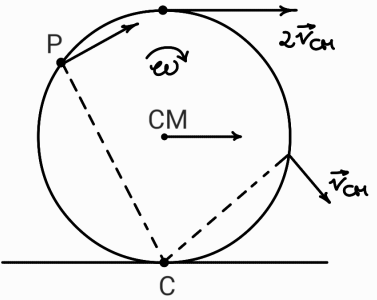
\includegraphics[width=0.4\linewidth]{Immagini/MPR.png}
    \caption{moto di puro rotolamento.}
    \label{fig: MPR}
\end{figure}
In ogni intervallo di tempo $dt$ il corpo che rotola senza strisciare può venir considerato come se ruotasse intorno ad un asse, fisso durante $dt$, passante per il punto di contatto $C$ e ortogonale al piano della figura \ref{fig: MPR}, con velocità angolare $\omega$. La velocità di ogni punto del corpo di conseguenza è ortogonale alla linea che congiunge $C$ con il punto ed è in modulo proporzionale alla distanza da $C$, quindi $v_P=\omega\overline{PC}$. In un intervallo successivo $dt$ il contatto avviene in un altro punto $C'$, infinitamente vicino $C$, e si ripete la rotazione attorno ad un altro asse fisso passante per $C'$, e così via. La velocità del punto $C$, distante $\vr$ dal centro di massa, si può sempre scrivere come $\vv_C=\vcm+\vom\times\vr$, mentre la condizione di puro rotolamento implica che $\vcm=-\vom\times\vr$. In modulo quindi si hanno
\begin{equation}
    v_{CM}=\omega r,\quad a_{CM}=\alpha r.
\end{equation}
Nel moto di puro rotolamento esiste una precisa relazione tra la velocità con cui avanza il centro di massa e  la velocità angolare, pertanto non sono indipendenti. Nel complesso la successione di rotazioni infinitesime attorno a $C$ equivale ad una rototraslazione in cui il centro di massa avanza con velocità $v_{CM}$ mentre il corpo ruota con velocità angolare $\omega$ rispetto ala centro di massa. 

Si consideri allora il caso di un corpo di massa $m$ e raggio $r$ che rotola senza strisciare su un piano orizzontale sotto l'azione di una forza orizzontale $\vF$ costante applicata all'asse. Sul corpo agisce anche la forza peso $m\vg$ e la reazione del piano $\vR$, che ha una componente normale $\vN$ e una tangenziale $\bm{f}$ corrispondente alla forza di attrito statico. La legge del moto del centro di massa è
\begin{equation}
    \vF+\vR+m\vg=m\acm,
\end{equation}
che proiettata sugli assi $x$ e $y$ restituisce rispettivamente
\begin{equation}
\label{eq: puro rot. 1}
    F-f=ma_{CM},\quad N=mg.
\end{equation}
Il teorema del momento angolare, scelto il centro di massa $O$ come polo, si scrive
\begin{equation}
    \vM=\vr\times\bm{f}=I\valpha,
\end{equation}
il cui modulo è
\begin{equation}
\label{eq: puro rot. 2}
     rf=I\alpha=I\frac{a_{CM}}{r}.
\end{equation}
Facendo sistema tra \eqref{eq: puro rot. 2} e la proiezione sull'asse $x$ \eqref{eq: puro rot. 1} si ricavano
\begin{equation}
    a_{CM}=\frac{F}{m\bigg(1+\dfrac{I}{mr^2}\bigg)},\quad f=\frac{F}{1+\dfrac{mr^2}{I}}.
\end{equation}
La forza $f$ non può assumere qualsiasi valore: non deve superare la massima forza di attrito statico, ovvero deve essere soddisfatta la disuguaglianza
\begin{equation}
    f\le\mu_sN=\mu_smg\Rightarrow F\le\mu_smg\bigg(1+\dfrac{mr^2}{I}\bigg)=F_{lim}.
\end{equation}
Pertanto, il moto può essere di puro rotolamento solo se la forza applicata non supera questa valore limite, altrimenti il corpo rotola e striscia. 

Invece di spingere il corpo, si può applicare all'asse un momento costante $\vM$. In questo caso, l'azione di $\vM$ tende a far slittare verso sinistra il punto di contatto e $\bm{f}$ è ora rivolta verso destra. Dalle equazioni
\begin{equation}
    \vR+m\vg=m\acm,\quad\vM+\vr\times\bm{f}=I\valpha,
\end{equation}
passando ai moduli si hanno
\begin{equation}
    N=mg,\quad f=ma_{CM},\quad M-rf=I\frac{a_{CM}}{r},
\end{equation}
da cui si ricavano
\begin{equation}
    a_{CM}=\frac{M}{mr^2\bigg(1+\dfrac{I}{mr^2}\bigg)},\quad f=\frac{M}{r\bigg(1+\dfrac{I}{mr^2}\bigg)}.
\end{equation}
Anche in questo caso si deve verificare
\begin{equation}
    f\le\mu_sN=\mu_smg\Rightarrow M\le\mu_smgr\bigg(1+\frac{I}{mr^2}\bigg)=M_{lim}.
\end{equation}
Mentre sotto l'azione di $\vF$ la reazione tangente $\bm{f}$ si oppone dal moto, a causa dell'azione di $\vM$, $\bm{f}$ favorisce il moto causando l'accelerazione del centro di massa. 

Nel caso più generale si ha l'azione contemporanea di una forza e di un momento. In tal caso non si può decidere a priori la direzione della forza $\bm{f}$, per cui la si assume parallela e concorde all'asse $x$. Le equazioni del moto sono
\begin{equation}
    F+f=ma_{CM},\quad M-rf=I\frac{a_{CM}}{r},
\end{equation}
da cui si ricavano
\begin{equation}
    a_{CM}=\frac{1}{m}\frac{F+\dfrac{M}{r}}{1+\dfrac{I}{mr^2}},\quad f=\frac{\dfrac{M}{r}-\dfrac{I}{mr^2}F}{1+\dfrac{I}{mr^2}}.
\end{equation}
con $f\le\mu_sN=\mu_smg$. La forza di attrito risulta concorde o discorde rispetto all'asse $x$ a seconda che $M$ sia maggiore o minore di $IF/mr$. In particolare, se $M=IF/mr$, la forza $f$ è nulla e $a_{CM}=F/m$: è possibile un moto accelerato anche in assenza di attrito. 

In conclusione, nel moto di rotolamento di un corpo rigido è possibile, con opportuni valori delle forze e dei momenti esterni, realizzare le condizioni per cui la reazione del piano è tale da mantenere fermo il punto di contatto., così che il corpo rotola senza strisciare. 

\subsubsection{Conservazione dell'energia e attrito volvente}
Al moto di puro rotolamento sotto l'azione di forze conservative si può applicare il principio di conservazione dell'energia meccanica. Infatti, la forza di attrito, che è normalmente diversa da zero, agisce su un punto fermo per cui lo spostamento è nullo e quindi è nullo il lavoro. Tuttavia, la conservazione dell'energia meccanica è un caso limite: sperimentalmente un corpo che rotola senza strisciare, in assenza di forze e momenti applicati, si arresta dopo un certo tempo. Pertanto, esiste un'altra forma di attrito, detta attrito volvente, che viene attribuito alla deformazione locale del piano ed è schematizzato con l'azione di un momento $M_v=hmg$ che si oppone al moto, dove $h$ è il coefficiente di attrito volvente. Per vincere tale momento, si deve applicare al corpo di massa $m$ e raggio $r$ una forza di trazione tale che $F\ge hmg/r$.
\begin{obs}
    Dato che l'effetto dell'attrito volvente è minimo rispetto a quello radente e dinamico, nel seguito lo si trascura.
\end{obs}

\subsection{Impulso angolare}
Come visto, la forma integrale del secondo principio di Newton è esprimibile tramite il teorema dell'impulso: l'impulso della forza è uguale alla variazione della quantità di moto. In modo analogo, si deduce il seguente teorema.
\begin{teo}[teorema dell'impulso angolare]
    L'azione di un momento durante un intervallo finito di tempo causa una variazione finita del momento angolare
    \begin{equation}
        \int_{t_1}^{t_2}\vM\,dt=\vL(t_2)-\vL(t_1)=\Delta\vL.
    \end{equation}
\end{teo}
Un modo per mettere in rotazione un corpo rigido rispetto ad un asse fisso consiste nell'applicazione di una forza intensa per un tempo molto breve in un dato punto. Prendendo come polo il punto di sospensione $O$ del corpo si ha
\begin{equation}
    \int\vM\,dt=\int(\vr\times\vF)\,dt=\vr\times\int\vF\,dt=\vr\times\vJ=\Delta\vL.
\end{equation}
Quindi, l'applicazione dell'impulso provoca, oltre ad una variazione di quantità di moto, una variazione di momento angolare uguale al momento dell'impulso. Si noti che nell'integrale non compaiono le forze di attrito, dato che hanno momento nullo in quanto applicate in $O$, e nemmeno la forza peso in quanto si assume trascurabile il suo impulso angolare rispetto a quello di $\vF$.
\begin{obs}
    Si erano già trovate espressioni analoghe e formalmente identiche per il punto materiale. La principale differenza sta nell'espressione del momento angolare.
\end{obs}

\subsection{Leggi di conservazione}
Se la risultante delle forze esterne è nulla, il centro di massa si muove di moto rettilineo uniforme, ma il moto dei singoli punti non è detto sia traslatorio rettilineo uniforme. In tal caso, la quantità di moto $\vp$ è costante e di conseguenza anche $\vcm$ è costante, con $\vp=m\vcm$. 

Assumendo come polo un punto fisso in un sistema di riferimento inerziale o il centro di massa, se $\vM=0$, allora il momento angolare $\vL$ resta costante in modulo, direzione e verso. Questo però non comporta $\vom=costante$, in quanto non è detto che il moto di rotazione avvenga attorno ad un asse principale di inerzia, ovvero che sia $\vL=I\vom$.

La legge di conservazione dell'energia meccanica nel moto di un corpo è valida quando non ci sono attriti o quando, come nel moto di puro rotolamento, le forze di attrito non compiono lavoro, pur essendo presenti. Inoltre, le reazioni vincolari che tengono fissi uno o più punti, non compiono lavoro, mentre la presenza di momenti di attrito che agiscono sull'asse di rotazione determina un lavoro che provoca una diminuzione dell'energia meccanica. 

\subsection{Equilibrio statico}
La condizione di equilibrio statico per un punto materiale è che la risultante delle forze applicate al punto sia nulla, ossia $\vR=0$. Se il punto è inizialmente in quiete, rimane in tale stato. Per un corpo rigido inizialmente in quiete si ha l'equilibrio statico se
\begin{equation}
    \vR=0,\quad\vM=0.
\end{equation}
La prima realizza l'equilibrio statico del centro di massa, ossia $\vcm=0$, mentre con la seconda non si ha moto rotatorio, ossia $\vom=0$. In questo caso, $\vM$ è indipendente dal polo, quindi se quest'ultimo è nullo rispetto ad un polo, lo è rispetto a qualsiasi altro. 

Si consideri infine l'equilibrio dei corpi sospesi, tipo pendolo composto, sottoposti alla forza peso. In qualsiasi posizione in cui il centro di massa non si trova sulla verticale passante per il centro di sospensione $O$, il momento della forza peso rispetto ad $O$ è diverso da zero e si compone di un'accelerazione angolare. Il centro di massa ha accelerazione diversa da zero, determinata dalla risultante della forza peso e della reazione vincolare in $O$. In tal caso non può esserci equilibrio statico se non agiscono altre forze. Se invece il centro di massa sta sulla verticale passante per $O$ e ha velocità nulla, la posizione è di equilibrio: il momento è nullo e la risultante delle forze è nulla (la reazione vale $m\vg$). Ci sono due posizioni possibili di questo tipo: il centro di massa sta sotto oppure sopra $O$. Nel primo caso se si allontana il corpo dalla posizione di equilibrio la forza peso tende a riportarlo, per cui l'equilibrio è stabile; nel secondo caso, il corpo si allontana ulteriormente dalla posizione di equilibrio, la forza peso lo fa ruotare portandolo verso il basso con il centro di massa sotto $O$, per cui l'equilibrio è instabile. Se il centro di sospensione coincide con il centro di massa, il momento della forza peso sarebbe sempre nullo e il corpo starebbe in quiete in qualsiasi posizione angolare: l'equilibrio è indifferente. 